% \section{Background: AllReduce, AllGather, and Point-to-Point communication}
% \label{app:collective-background}

% In this section, we provide details of the communication patterns used in tensor, pipeline and data parallelism strategies. 
% %\sys{} extends the model tree abstraction of IrEne by introducing a dedicated module for AllReduce operations, which is essential for capturing the energy dynamics of tensor-parallelized inference. This extension is necessary because AllReduce operations introduce unique energy consumption patterns tied to inter-GPU communication that cannot be captured by the existing math, ML, or module level nodes.

% \subsection{AllReduce in tensor parallelism}
% \label{app:tp-ar}

% Tensor parallelism uses a ring-based communication pattern. In the ring AllReduce algorithm, GPUs are arranged in a logical ring structure where each GPU communicates only with its immediate neighbors, reducing global communication overhead. The operation proceeds in two distinct phases:

% \begin{enumerate}
%     \item \textbf{ReduceScatter Phase}: Each GPU divides its data into equal chunks (one per GPU). In this phase, each GPU sends a chunk to its successor in the ring and receives a chunk from its predecessor. Upon receiving data, each GPU performs a reduction operation (e.g., sum) with its corresponding local chunk. This process continues for $n-1$ steps (where $n$ is the number of GPUs), at which point each GPU has one fully reduced chunk of the final result.
    
%     \item \textbf{AllGather Phase}: In this phase, the reduced chunks are disseminated to all GPUs. Each GPU sends its reduced chunk to its successor and receives a different reduced chunk from its predecessor. After $n-1$ steps, all GPUs have all chunks of the fully reduced data.
% \end{enumerate}

%There are two phases of the AllReduce process that is captured by the model abstraction tree:
%
%\begin{enumerate}
%    \item \textbf{Communication Nodes}: Capturing the data transfers between adjacent GPUs in the ring.
%    \item \textbf{Synchronization Nodes}: Modeling the waiting periods where faster GPUs idle while waiting for slower ones to complete their operations.
%\end{enumerate}

% \subsection{Point-to-Point Data Transfers in Pipeline Parallelism}
% \label{app:pp-p2p}

% In pipeline parallelism, stage $i$ sends its forward activations to stage $i{+}1$ via \emph{point-to-point} device-to-device transfers (e.g., NVLink/PCIe/Ethernet). 
% During inference there are no gradients; the only communication are the hop-local activation sends/receives. 
% Operationally, the transfer for a given microbatch occurs immediately after stage $i$ finishes its forward compute and before stage $i{+}1$ launches its first kernel on the received activations. 
%We profile this communication by timestamping (with \texttt{nsys}) the end of stage~$i$’s last forward kernel and the start of stage~$i{+}1$’s first forward kernel; the interval between these two events is attributed to the Point-to-Point transfer. 
%We integrate power over this window to obtain P2P energy, repeating across hops and microbatches to form robust aggregates. Because these are explicit, hop-local sends/recvs rather than collectives, timing variability is typically small, and the attribution is more deterministic than in tensor-parallel synchronization phases.


% \subsection{All Gather in data parellelism}
% \label{app:dp-allgather}

% In data parallelism, each replica computes the full forward pass for its local microbatch and then \emph{collates the final outputs} (e.g., logits/token scores) across replicas with a single AllGather at the end of inference. Mechanistically, the last layer on each GPU (typically the output projection / logits head) finishes, the runtime immediately exchanges each replica’s output tensor, and the concatenated result is handed to the host for post-processing (sampling, metrics, or write-out). 
%This makes profiling straightforward: \emph{profiling the output layer automatically profiles the AllGather}, since it is the next and final step. 
%This collation is a \emph{single, tail-end} exchange of \emph{final outputs} (logits/token scores) whose tensors are much smaller than hidden activations, and it happens once per request (or per decode step). 
    % By contrast, Pipeline P ships \emph{activations between every adjacent stage} for each microbatch, and TP executes \emph{layer-internal collectives} (e.g., reduce–scatter/all-gather) on large hidden states multiple times per layer—hence substantially higher communication volume and energy in PP/TP than in DP.


\section{Methodology: Data Collection to predict communication energy}
\label{app:data-collection-parallel}
We describe the methodology we use to collect data to build a communication energy prediction model. Since communication is different for different parallelism strategies, we describe our data collection method for each parellism strategy below.

\paragraph{Tensor Parallelism (TP)}: During profiling, we capture the \emph{full distribution} of energy consumption caused by non-deterministic GPU synchronization through multiple runs. 
  By capturing a distribution of GPU wait times, rather than relying on a single execution run, we ensure that \sys{} reflects both leading and lagging GPU behavior, \be{accounting for variability}.
  We specifically capture the distribution of 
  %NCCL's (Nvidia Collective Communication Library) ring 
  the ring \textbf{AllReduce} operation, which consists of (i) ReduceScatter: GPUs exchange neighbor chunks and reduce for $n{-}1$ steps until each holds one fully-reduced shard, followed by (ii) AllGather: GPUs circulate these shards for $n{-}1$ steps so all ranks recover the full tensor. 
  The abstraction includes both \emph{communication} (hop transfers) and \emph{synchronization} (idle/wait due to stragglers), since AllReduce energy is shaped by link activity and barrier-induced stalls.

\paragraph{Pipeline Parallelism (PP)}: We capture data transfer by benchmarking the interval between completion of boundary layer in the producing stage and start of the next stage in the next GPU. 
    The only inference-time communication is \textbf{point-to-point} (P2P) activation transfers from stage $i$ to $i{+}1$ after stage $i$ finishes its forward kernels and before stage $i{+}1$ starts compute on received activations. 
    We profile each hop by timestamping (via \texttt{nsys}) the end of stage $i$’s last forward kernel and the start of stage $i{+}1$’s first forward kernel; the intervening interval is attributed to P2P transfer, and power is integrated over this window to estimate P2P energy.

\paragraph{Data Parallelism} Since each replica produces its own output, profiling the final output stage (\textbf{AllGather}) is sufficient to capture communication energy. Replicas run full forward passes independently and perform a single tail-end AllGather operation to collate final outputs (e.g., logits/token scores) across GPUs; this exchange occurs immediately after the output layer completes, making attribution straightforward and typically lower-volume than TP/PP communication.

\section{Methodology: Features}
\label{appendix:features}

\begin{table}[t]
\centering
\small
\setlength{\tabcolsep}{4pt}
\renewcommand{\arraystretch}{1.05}

\begin{tabular}{@{}
>{\raggedright\arraybackslash}p{0.48\linewidth}
>{\raggedright\arraybackslash}p{0.48\linewidth}
@{}}
\toprule
\rowcolor{rowblue}
\multicolumn{2}{@{}l@{}}{\textbf{Resource Utilization Features}}\\
\midrule
CPU utilization (\%) & CPU mem. utilization (\%)\\
\rowcolor{rowblue} GPU utilization (\%) & GPU mem. utilization (\%)\\
CPU clock (GHz) & CPU mem. clock (GHz)\\
\rowcolor{rowblue} Memory (bytes) & GPU clock (GHz)\\
GPU mem. clock (GHz) & \\
\midrule

\rowcolor{rowblue}
\multicolumn{2}{@{}l@{}}{\textbf{Execution Features}}\\
\midrule
Batch size & Sequence length\\
\rowcolor{rowblue} FLOPs per token (billions) & Execution time (s)\\
GPU energy NVML (Wh) & Number of GPUs\\
\midrule

\rowcolor{rowblue}
\multicolumn{2}{@{}l@{}}{\textbf{Model Structure Features}}\\
\midrule
Feed-forward dimension & Transformer blocks\\
\rowcolor{rowblue} Hidden embedding size & Attention heads\\
Key-value heads & \\
\midrule

\rowcolor{rowblue}
\multicolumn{2}{@{}l@{}}{\textbf{Communication Features}}\\
\midrule
Bytes transferred & Effective bandwidth \\
% \rowcolor{rowblue} Hidden embedding size & Attention heads\\

\bottomrule
\end{tabular}
\vspace{-9pt}
\caption{Features used by \sys{} for prediction.}
\label{tab:features}
\vspace{-17pt}
\end{table}

Table~\ref{tab:features} summarizes these features, grouped into resource utilization (captures system- and device-level activity during inference), execution parameters (capture the workload configuration that drives runtime/energy), and model structure (captures architectural properties that determine tensor sizes). 
For communication modules, we additionally collect communication-specific features: the bytes sent, the bytes received, and the effective bandwidth for each inter-GPU communication event.

% \section{Methodology Alpha--Beta Model for Communication Energy}
% \label{app:alpha-beta-comm}
% \aruna{can potentially be removed, content is moved to main text}
% {
% PIE-P models collective communication using an offline-calibrated alpha--beta latency predictor. For a communication event $e$ of operation type $o$ running on $p$ GPUs, let $B_{e}^{\mathrm{out}}$ and $B_{e}^{\mathrm{in}}$ denote the bytes sent and received by each rank. The total per-rank communication volume is:
% }
% \begin{equation}
% \label{eq:comm-volume}
% V_e =
% B_{e}^{\mathrm{out}} + B_{e}^{\mathrm{in}} .
% \end{equation}
% The communication latency is then predicted as
% \begin{equation}
% \label{eq:alpha-beta-comm}
% T*{e}^{\mathrm{comm}} =
% \alpha*{o,p} + \beta_{o,p} V_e .
% \end{equation}
    % {}
% Here, $\alpha_{o,p}$ captures fixed launch, scheduling, and synchronization overheads, while $\beta_{o,p}=1/B_{o,p}^{\mathrm{eff}}$ captures the inverse effective bandwidth. For ring AllReduce with tensor size $S_e$, each rank sends and receives $(p-1)S_e/p$ bytes. Thus, the AllReduce communication volume is
% \begin{equation}
% \label{eq:allreduce-volume}
% V_e^{\mathrm{AR}} =
% \frac{2(p-1)}{p}S_e .
% \end{equation}
% The AllReduce latency prediction is
% \begin{equation}
% \label{eq:allreduce-latency-short}
% T*{e}^{\mathrm{AR}} =
% \alpha*{\mathrm{AR},p}
% +
% \beta_{\mathrm{AR},p} V_e^{\mathrm{AR}} .
% \end{equation}

% PIE-P converts predicted communication latency into energy using calibrated average communication power. For an AllReduce event, the predicted energy is
% \begin{equation}
% \label{eq:allreduce-energy-short}
% E*{e}^{\mathrm{AR}} =
% \frac{P*{\mathrm{AR},p}^{\mathrm{comm}}
% T*{e}^{\mathrm{AR}}}{3600}.
% \end{equation}
% The total compute and communication energies are
% \begin{equation}
% \label{eq:total-compute-energy-short}
% E^{\mathrm{compute}} =
% \sum*{m \in \mathcal{M}}
% E*{m}^{\mathrm{compute}} .
% \end{equation}
% \begin{equation}
% \label{eq:total-comm-energy-short}
% E^{\mathrm{comm}} =
% \sum*{e \in \mathcal{C}}
% E*{e}^{\mathrm{comm}} .
% \end{equation}
% The final model-level prediction is
% \begin{equation}
% \label{eq:model-energy-alpha-beta-short}
% E*{\mathrm{model}} =
% R\left(
% E^{\mathrm{compute}} +
% E^{\mathrm{comm}}
% \right).
% \end{equation}
% This formulation captures both the fixed overhead and message-size-dependent cost of inter-GPU communication without requiring online communication-energy sampling during inference.

\section{Methodology: Details of predicting communication energy}
\label{app:alpha-beta-comm}

Section~\ref{ss:design-communication} introduces the $\alpha$-$\beta$ communication model used by \sys{} in Eq.~\ref{eq:comm-latency-main}. 
Here, we provide the details for computing the communication-volume term $\left(B_{e}^{\mathrm{out}} + B_{e}^{\mathrm{in}}\right)$ and the effective-bandwidth parameter $\beta_{o,p}$ used in that equation.

For a communication event $e$ of operation type $o$ running on $p$ GPUs, let $B_{e}^{\mathrm{out}}$ and $B_{e}^{\mathrm{in}}$ denote the bytes sent and received by each GPU. 
The total per-GPU communication volume is:
\vspace{-9pt}
\begin{equation}
\label{eq:comm-volume}
V_e =
B_{e}^{\mathrm{out}} + B_{e}^{\mathrm{in}} .
\vspace{-9pt}
\end{equation}

We calibrate the effective bandwidth offline for each communication operation $o$ and GPU count $p$. 
For each calibration run, we record the communication volume $V_e$ and the observed communication time $T_{e}^{\mathrm{obs}}$. 
We then fit the alpha-beta relation:
\vspace{-9pt}
\begin{equation}
\label{eq:alpha-beta-calibration}
T_{e}^{\mathrm{obs}} =
\alpha_{o,p} +
\beta_{o,p} V_e .
\vspace{-9pt}
\end{equation}
Here, $\alpha_{o,p}$ captures fixed communication overheads, while $\beta_{o,p}$ captures the message-size-dependent transfer cost. 
The corresponding effective bandwidth is:
\vspace{-9pt}
\begin{equation}
\label{eq:effective-bandwidth}
B_{o,p}^{\mathrm{eff}} =
\frac{1}{\beta_{o,p}} .
\vspace{-9pt}
\end{equation}

For ring AllReduce, if the communicated tensor has size $S_e$ bytes, each GPU sends and receives $(p-1)S_e/p$ bytes across the ReduceScatter and AllGather phases. 
Thus, the total per-GPU AllReduce communication volume is:
\vspace{-9pt}
\begin{equation}
\label{eq:allreduce-volume}
V_e^{\mathrm{AR}} =
\frac{2(p-1)}{p}S_e .
\vspace{-9pt}
\end{equation}
This volume is used as the communication-volume input for AllReduce events in Eq.~\ref{eq:comm-latency-main}. 
For pipeline-parallel point-to-point transfers and data-parallel AllGather operations, we apply the same accounting procedure using the tensor size and the corresponding communication pattern described in Appendix~\ref{app:collective-background}.


\section{Methodology: Training }
\label{app:training_methodology}

Our detailed training methodology is described below. We use a hierarchical approach, first training module-level predictors and then combining them for model-level prediction. We employed 3-fold cross-validation at the module level, training on 70\% of datapoints while testing on the remaining 30\%. 

Each module (e.g., Self-Attention, MLP, AllReduce) is sampled $10{,}000$ times to build a robust dataset. A single sample corresponds to one aggregated measurement obtained by running the module $100{,}000$ times in a specific GPU configuration setting. For each sampling run, we compute the mean, standard deviation, minimum, and maximum values of these features across all participating GPUs to account for runtime variance and workload imbalance. These are combined with structural features to form the complete feature vector for each sample.

To ensure that the models are evaluated under varied operational conditions, we perform sampling across multiple output configurations. Specifically, for each model variant, we run experiments using batch sizes of 8, 16, 32, and 64, and output sequence lengths of 512 and 1024. This sampling regime captures both low and high throughput scenarios, improving the robustness and generalizability of our predictors. We use Deepspeed \citep{deepspeed}, a widely used inference serving python library to run our tests for all parallelism modalities.


For each model family (e.g., Vicuna), we combined module-level energy predictions across all variants using the extracted features. The model-level energy prediction was composed using the regression formula: 
% $\text{model\_energy} = \text{regression}(\text{self\_attention\_energy} + \text{MLP\_energy} + \text{AllReduce\_energy} + \ldots)$.


\vspace{-9pt}
\setlength{\abovedisplayskip}{2pt}
\setlength{\belowdisplayskip}{2pt}
\begin{equation}
\begin{aligned}
E_{\text{model}} = \mathcal{R}(&E_{\text{attn}} + E_{\text{MLP}} \\
&+ E_{\text{AllReduce}} + \ldots)
\end{aligned}
\vspace{-6pt}
\end{equation}
% \vspace{-9pt}

%For the \sys{} without waiting phase baseline, we substituted the AllReduce module's predicted energy with just the network transfer predicted energy, excluding the waiting phase component. For the IrEne baseline, we excluded AllReduce energy completely from the regression. 
%\label{app:use-case-ground-truth}

%Figure~\ref{fig:mape_comparison} reports the MAPE values obtained from this regression, where each model-level energy prediction MAPE is derived from a regression over its module-level energy components. The error bars represent the standard errors computed over the individual percentage errors of each prediction.



%\label{app:module_mape}
%For each model variant, we obtain module-level energy MAPE values (in Table ~\ref{tab:module_mape_comparison} by running each module type (e.g., Self-Attention, MLP, AllReduce) multiple times under varying input configurations and computing their predicted energy values. If a module appears multiple times in a model (e.g., multiple Feed Forward Networks), we first average the predicted energies across those instances. The final MAPE for a module type is then averaged across all variants and across all four model families.

%\begin{figure}[t]
 %   \centering
  %  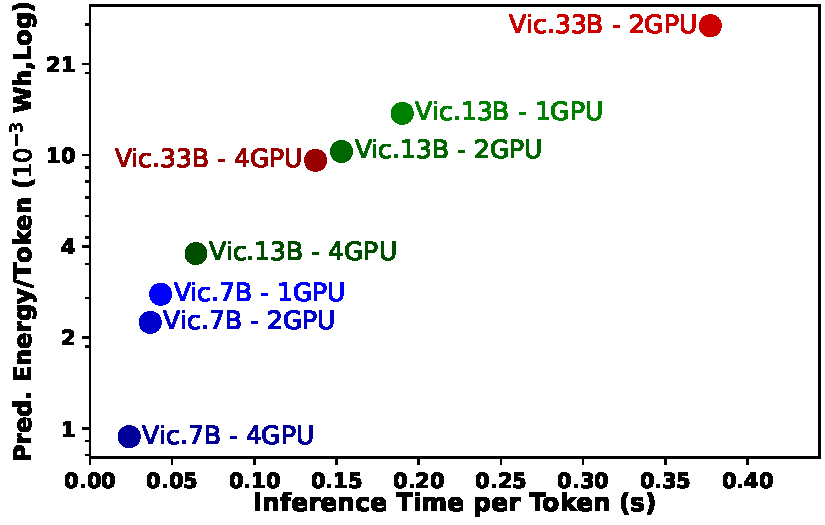
\includegraphics[width=\columnwidth]{figures/pareto_plot.pdf}
  %  \caption{Ground truth energy trade-off between inference time per token and energy per token (on log scale) for Vicuna under tensor parallelism.}
  %  \label{fig:pareto_plot_ground_truth}
%\end{figure}
%Figure~\ref{fig:pareto_plot_ground_truth} shows the trade-off between actual energy consumption and inference time per token across Vicuna model sizes and GPU configurations.
%\label{app:generalization-unseen-variants}

To evaluate generalization across unseen model variants (Appendix~\ref{app:additional-generalization-unseen-variants}), we adopt a leave-one-variant-out strategy. Specifically, for each experiment, we exclude one model variant entirely from training and train a model-level energy regressor using the predicted module-level energies from the remaining variants within the same model family. During evaluation, we predict the total energy of the held-out variant using its module-level energy predictions as input. This setup allows us to assess the ability of \sys{} to generalize across model scales and configurations within a family.




\section{Evaluation: Baselines}
\label{app:baselines}

In this section, we describe the baselines we use to compare with \sys{} in more detail. 

\textbf{IrEne}~\citep{irene} is a multi-level energy prediction model that combines fine-grained model execution features with resource utilization for more accurate energy prediction.  
IrEne first constructs a model tree abstraction that captures the model's computational structure at three levels: math level, machine learning (ML) level, and module level. 
The math level consists of basic mathematical operations like matrix multiplication and addition, which are model-agnostic and can generalize across various models. 
The operations at the ML level nodes, such as Linear and LayerNorm, are more specific to ML tasks but are still generalizable. 
The module level nodes (e.g., SelfAttention) are higher-level nodes that are made up of several ML tasks combined together. 

 
IrEne then uses a bottom-up prediction approach for energy estimation. At the leaf level, IrEne learns the energy consumption of each node using features derived from runtime resource utilization (e.g., GPU usage) and model specifications (e.g., input size). IrEne uses ground truth measurement for training. At each intermediate node going up to the root, energy predictions are recursively computed by combining the predicted energy values of child nodes through a single regressor.

\textbf{CodeCarbon}: Software based energy estimator that tracks runs via readily available telemetry (e.g., GPU via NVML, CPU via RAPL/powermetrics) and integrates power over time to report kWh (and optionally emissions). CodeCarbon is currently state-of-the-art for software-based energy estimation and is used by researchers and practitioners for system-level energy/emissions estimation~\cite{Jesse-dodge-icml}.

\textbf{Wilkins et. al}: Energy estimator that learns coefficients based on token-in/token-out energy ratios. We implement this token-in/token-out regression technique, illustrated in  
%which predicts per-request energy as a function of input and output token counts with an interaction term in 
Eq.~(\ref{eq:wilkins-tok2e}), where the coefficients $(\alpha_0,\alpha_1,\alpha_2)$ are fit from a calibration set. This is included as a recent, deployment-friendly baseline that estimates energy without hardware monitors. 
% \begin{wrapfigure}[3]{r}{0.48\linewidth}
% 
% \begin{minipage}{\linewidth}
% \setlength{\abovedisplayskip}{4pt}\setlength{\belowdisplayskip}{4pt}
\vspace{-6pt}
\setlength{\abovedisplayskip}{2pt}
\setlength{\belowdisplayskip}{2pt}
\begin{equation}
\begin{aligned}
e_K(\tau_{\mathrm{in}}, \tau_{\mathrm{out}})=\;&\alpha_0\,\tau_{\mathrm{in}}+\alpha_1\,\tau_{\mathrm{out}}
+\alpha_2\,\tau_{\mathrm{in}}\tau_{\mathrm{out}}
\end{aligned}
\label{eq:wilkins-tok2e}
\vspace{-6pt}
\end{equation}
% \vspace{-9pt}

\textbf{NVML}: NVML is a software based GPU status tracking software that allows for real time metrics such as temperature, power, and memory utilization. We implement a linear regressor at the model level using NVML-collected energy as the independent variable and total energy consumed as the dependent variable. 



%\section{Additional results: AllReduce energy consumption }
%\label{app:allreduce-energy}
%
%\begin{figure*}[t]
%\centering
%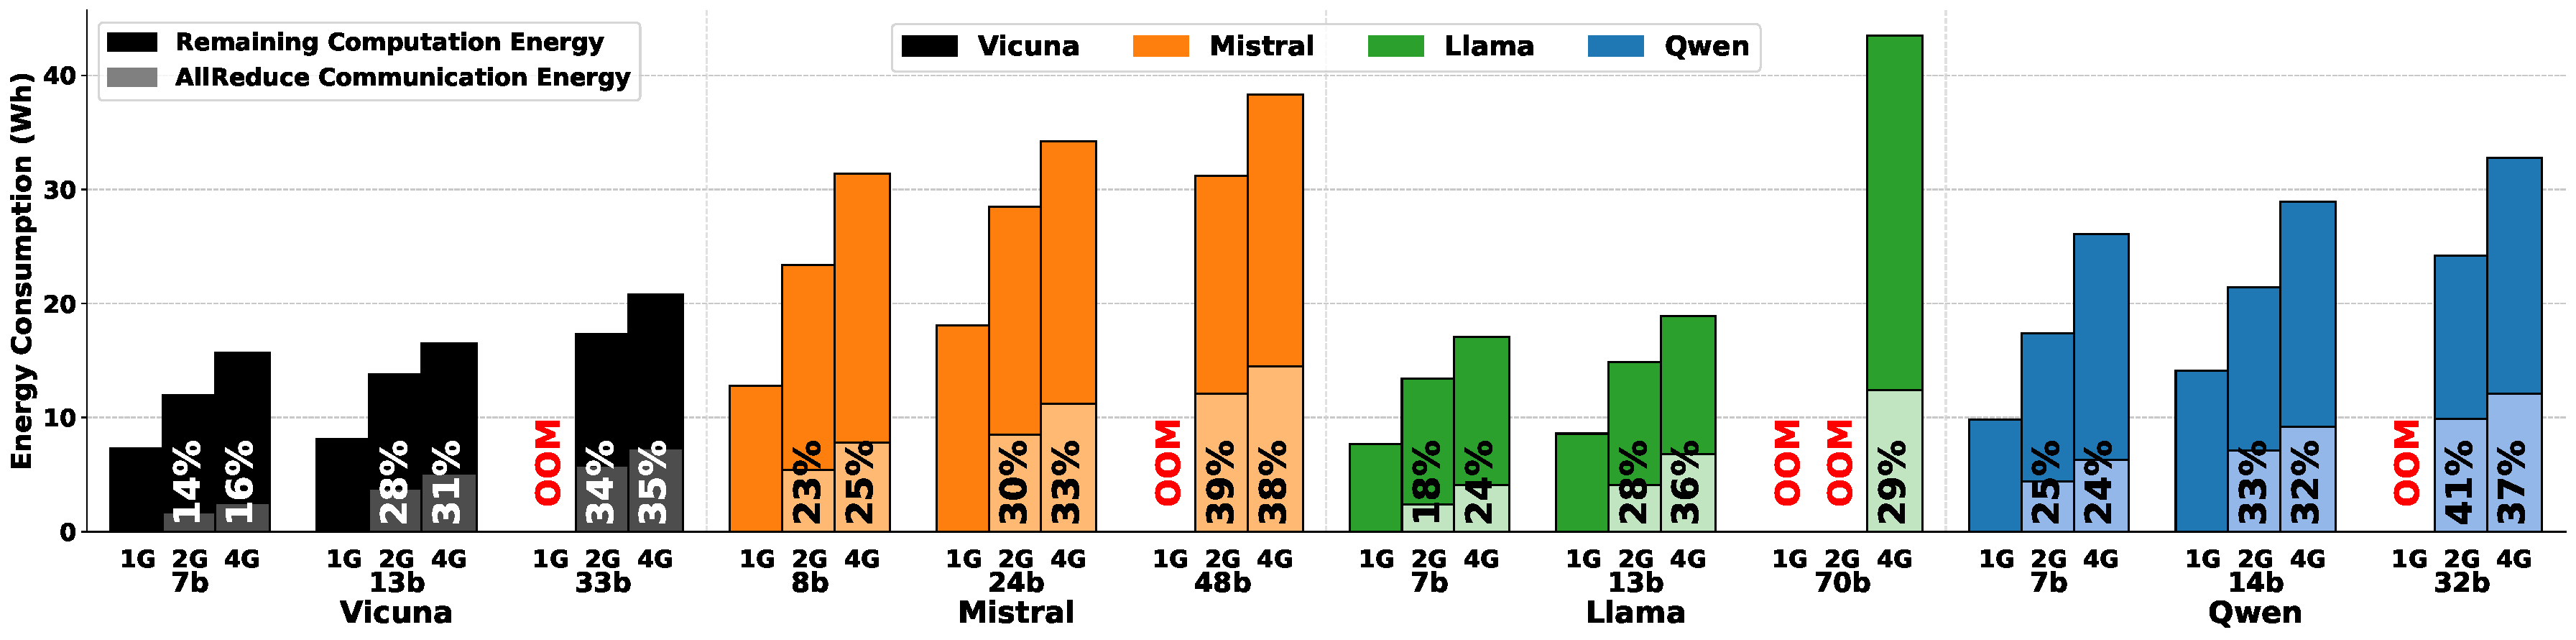
\includegraphics[width=\textwidth]{figures/llm_energy_comparison.pdf}
%\caption{Energy consumption across different model families and GPU configurations. The bars show total energy consumption per model with lighter-colored segments representing AllReduce communication energy (\% shown) and darker segments showing remaining computation energy.}
%\label{fig:all_reduce_ratio}
%\vspace{-6pt}
%\end{figure*}
%
%
%Figure~\ref{fig:all_reduce_ratio} shows the energy consumption breakdown for parallelized inference across different GPU configurations for four model families: Vicuna, Mistral, Llama, and Qwen. Across all model families, AllReduce consumes a considerable amount of energy both for 2 to 4 GPUs in tensor-parallel configurations for batched inferences. For example, for the Vicuna family, the AllReduce energy constitutes 14.2\% (1.7 Wh/12.0 Wh) of total energy with 2 GPUs for the 7B model, increasing to 15.9\% (2.5 Wh/15.7 Wh) with 4 GPUs. This proportion is higher for larger models, reaching 27.5\% (5.8 Wh/17.3 Wh) for Vicuna-33B with 2 GPUs and 35.1\% (7.3 Wh/20.8 Wh) with 4 GPUs.
%
%We observe that the proportion of AllReduce energy correlates strongly with the complexity of the transformer architecture. Models with more sophisticated attention mechanisms and larger feed-forward dimensions, such as Mistral and Qwen, show significantly higher AllReduce energy proportions compared to models with simpler architectures like Vicuna. More complex transformer blocks lead to higher AllReduce energy proportions because they generate larger intermediate tensors that must be synchronized across GPUs. 
%For instance, Mistral-8B employs grouped-query attention with 32 attention heads but only 8 key-value heads, resulting in approximately 245 GFLOPs per transformer block—31\% higher than Vicuna-7B's 187 GFLOPs per block with standard self-attention and 32 attention heads. As a result, the proportional energy consumption of AllReduce for Mistral is higher.


% \section{Additional results: NVML generalization for energy prediction}
% \label{app:nvml_generalization}
% \begin{table}[t]
% \centering
% \small
% \setlength{\tabcolsep}{3pt}
% \renewcommand{\arraystretch}{1.05}

% \begin{tabular}{
%   @{}
%   l
%   c
%   l
%   c
%   @{}
% }
% \toprule
% \textbf{Model} & \textbf{MAPE} & \textbf{Model} & \textbf{MAPE} \\
% \midrule
% \rowcolor{rowblue} Vicuna 7B   & 48.3\% & Llama 7B   & 47.4\% \\
% Vicuna 13B                     & 51.1\% & Llama 13B  & 49.1\% \\
% \rowcolor{rowblue} Vicuna 33B  & 50.0\% & Llama 70B  & 53.4\% \\
% \midrule
% Mistral 8B                     & 57.3\% & Qwen 8B    & 51.1\% \\
% \rowcolor{rowblue} Mistral 24B & 52.1\% & Qwen 14B   & 49.2\% \\
% Mistral 48B                    & 51.3\% & Qwen 32B   & 56.5\% \\
% \bottomrule
% \end{tabular}

% \caption{Leave-one-out generalization results for NVML-based regression. Each row shows MAPE when using NVML measurements to predict total energy for a model excluded from training. The high error rates, ranging from 47.4\% to 57.3\%, demonstrate NVML's poor generalization capabilities.}
% \label{tab:nvml_loo}
% \end{table}

% Beyond examining NVML's limitations as a direct proxy for total energy, we also evaluated its generalization capabilities using leave-one-out cross-validation. Table~\ref{tab:nvml_loo} shows the results when NVML-based regression models are trained on all models of the same model family except one, then tested on the excluded model.

% The results reveal significantly higher prediction errors compared to both in-sample NVML prediction (29.8-44.2\% MAPE) and \sys{}'s leave-one-out performance (15.8-24.5\% MAPE). MAPE values range from 47.4\% to 57.3\%, with an average of 51.5\% across all models (Table ~\ref{tab:nvml_loo}). These poor generalization results further reinforce our conclusion that GPU-only measurements are insufficient for accurate energy prediction in tensor-parallelized settings, particularly when generalizing to new model architectures or configurations. The substantial gap between \sys{} and NVML generalization performance (average improvement of 31.5 percentage points) demonstrates the critical importance of our approach's architecture-aware features and synchronization modeling.

\section{Additional results: NVML as a proxy for total energy}
\label{app:nvml_proxy}
\begin{table}[t]
\centering
\small
\setlength{\tabcolsep}{3pt}
\renewcommand{\arraystretch}{1.05}

\begin{tabular}{
  @{}
  l
  c
  l
  c
  @{}
}
\toprule
\textbf{Model} & \textbf{MAPE} & \textbf{Model} & \textbf{MAPE} \\
\midrule
\rowcolor{rowblue} Vicuna 7B   & 33.4\% & Llama 7B   & 31.1\% \\
Vicuna 13B                     & 31.4\% & Llama 13B  & 31.3\% \\
\rowcolor{rowblue} Vicuna 33B  & 29.8\% & Llama 70B  & 28.5\% \\
\midrule
Mistral 8B                     & 44.2\% & Qwen 8B    & 42.4\% \\
\rowcolor{rowblue} Mistral 24B & 40.3\% & Qwen 14B   & 38.0\% \\
Mistral 48B                    & 39.0\% & Qwen 32B   & 38.3\% \\
\bottomrule
\end{tabular}

\caption{MAPE when using NVML-reported GPU energy as a proxy for total system energy. This approach produces substantially higher errors compared to \sys{}. Experiments conducted on A6000s}
\label{tab:nvml_proxy}
\end{table}

Hardware vendors provide built-in power measurement interfaces such as NVIDIA Management Library (NVML) that report GPU-only energy consumption. Can these readily-available measurements be reliable proxies for total system energy through simple regression techniques? % potentially eliminating the need for specialized prediction frameworks. 
%To investigate this approach, we conducted an experiment using NVML-reported GPU energy values as the sole predictor for total system energy consumption.


Table~\ref{tab:nvml_proxy} shows the results when NVML is used to predict total energy. %Despite the apparent simplicity of using NVML measurements directly, 
Prediction errors across all model families and sizes are high. Vicuna models' MAPE range from 29.8\% to 33.4\%, while Mistral's are even higher between 39.0\% and 44.2\%. 
%NVML also generalizes poorly to unseen models, as shown in Appendix~\ref{app:nvml_generalization}.
%The result shows that tensor-parallelized inference energy involves complex interactions between computation, synchronization, and system-level dynamics that cannot be captured by GPU-only measurements alone. % In particular, NVML fails to account for several key factors: (1) CPU energy consumption during scheduling and orchestration, (2) detailed runtime metrics obtained through telemetry and tracing that reveal resource utilization patterns, and (3) model structural features that influence energy consumption across different tensor-parallel configurations. \sys{}'s superior performance demonstrates the necessity of a specialized prediction framework that explicitly models these tensor-parallelism-specific energy dynamics rather than relying on simplified proxy measurements.


%\section{Additional results: NVML generalization for energy prediction}
%\label{app:nvml_generalization}


\begin{table}[t]
\centering
\small
\setlength{\tabcolsep}{3pt}
\renewcommand{\arraystretch}{1.05}

\begin{tabular}{
  @{}
  l
  c
  l
  c
  @{}
}
\toprule
\textbf{Model} & \textbf{MAPE} & \textbf{Model} & \textbf{MAPE} \\
\midrule
\rowcolor{rowblue} Vicuna 7B   & 48.3\% & Llama 7B   & 47.4\% \\
Vicuna 13B                     & 51.1\% & Llama 13B  & 49.1\% \\
\rowcolor{rowblue} Vicuna 33B  & 50.0\% & Llama 70B  & 53.4\% \\
\midrule
Mistral 8B                     & 57.3\% & Qwen 8B    & 51.1\% \\
\rowcolor{rowblue} Mistral 24B & 52.1\% & Qwen 14B   & 49.2\% \\
Mistral 48B                    & 51.3\% & Qwen 32B   & 56.5\% \\
\bottomrule
\end{tabular}

\caption{Leave-one-out generalization results for NVML-based regression. Each row shows MAPE when using NVML measurements to predict total energy for a model excluded from training. The high error rates, ranging from 47.4\% to 57.3\%, demonstrate NVML's poor generalization capabilities. Experiments conducted on A6000s}
\label{tab:nvml_loo}
\end{table}

Beyond examining NVML's limitations as a direct proxy for total energy, we also evaluated its generalization capabilities using leave-one-out cross-validation. Table~\ref{tab:nvml_loo} shows the results when NVML-based regression models are trained on all models of the same model family except one, then tested on the excluded model.

The results reveal significantly higher prediction errors compared to both in-sample NVML prediction (29.8-44.2\% MAPE) and \sys{}'s leave-one-out performance (15.8-24.5\% MAPE). MAPE values range from 47.4\% to 57.3\%, with an average of 51.5\% across all models (Table ~\ref{tab:nvml_loo}). These poor generalization results further reinforce our conclusion that GPU-only measurements are insufficient for accurate energy prediction in tensor-parallelized settings, particularly when generalizing to new model architectures or configurations. The substantial gap between \sys{} and NVML generalization performance (average improvement of 31.5 percentage points) demonstrates the critical importance of our approach's architecture-aware features and synchronization modeling. These results were conducted on the A6000 hardware, but results were similar on the other two hardware. 


\section{Additional Results: Generalization across models}
\label{app:additional-generalization-models}

In practice, an energy predictor is most useful when it can be applied beyond the exact model and configuration it was trained on.
However, generalizing across entire model architectures is substantially more challenging than generalizing across configurations of the \emph{same} model because the energy-performance relationship can shift when the computation graph changes. 

To assess this capability, we perform a \emph{leave-one-family-out} evaluation: we exclude all measurements from one model family during training and then evaluate \sys{} on that held-out family under the same range of parallelization strategies and inference settings. 

Table~\ref{tab:cross_model_generalization} presents these cross-model results on the A6000 hardware.
When generalizing to the Vicuna family (first row in Table~\ref{tab:cross_model_generalization}), \sys{} achieves a MAPE of 24.1\%, compared to 49.3\% for IrEne, a relative improvement of 
51.1\%.
This pattern holds for all families. This result shows that \sys{} can leverage its compositional structure and featurization to extrapolate to unseen models. Table~\ref{tab:b40_cross_model_generalization} shows similar results for NVIDIA B40 hardware.

\begin{table}[t]
\centering
\small
\setlength{\tabcolsep}{4pt}
\renewcommand{\arraystretch}{1.05}
\begin{tabular}{lcc}
\hline
\textbf{Excluded Family} & \textbf{\sys{}} & \textbf{IrEne} \\
\hline
\rowcolor{rowblue}Vicuna  & 24.1\% & 49.3\% \\
Mistral                  & 27.0\% & 56.5\% \\
\rowcolor{rowblue}Llama  & 26.1\% & 55.3\% \\
Qwen                     & 27.6\% & 58.4\% \\
\hline
\end{tabular}
\caption{Cross-architecture generalization results on NVIDIA RTX A6000. Each row lists the model family excluded from training.}
\label{tab:cross_model_generalization}
\end{table}

\begin{table}[t]
\centering
\small
\setlength{\tabcolsep}{4pt}
\renewcommand{\arraystretch}{1.05}
\begin{tabular}{lcc}
\hline
\textbf{Excluded Family} & \textbf{\sys{}} & \textbf{IrEne} \\
\hline
\rowcolor{rowblue}Vicuna  & 13.2\% & 63.8\%  \\
Mistral                  & 15.1\% & 71.2\%  \\
\rowcolor{rowblue}Llama  & 23.1\% & 113.3\% \\
Qwen                     & 12.2\% & 62.9\%  \\
\hline
\end{tabular}
\caption{Cross-architecture generalization results on NVIDIA B40 GPUs. Each row lists the model family excluded from training.}
\label{tab:b40_cross_model_generalization}
\end{table}

\section{Additional Results: Generalization across variants}
\label{app:additional-generalization-unseen-variants}

\begin{table}[t]
\centering
\small
\renewcommand{\arraystretch}{1.05}
\begin{tabular}{lclc}
\hline
\textbf{Model} & \textbf{MAPE} & \textbf{Model} & \textbf{MAPE} \\
\hline
\rowcolor{rowblue}Vicuna 7B     & 15.84\% & Llama 7B      & 18.15\% \\
Vicuna 13B    & 17.72\% & Llama 13B     & 21.11\% \\
\rowcolor{rowblue}Vicuna 33B    & 17.55\% & Llama 70B     & 22.41\% \\
%Vicuna BS-16  & 16.89\% & Llama BS-16   & 18.33\% \\
%\rowcolor{rowblue}Vicuna BS-32  & 18.20\% & Llama BS-32   & 19.16\% \\
\hline
Mistral 8B    & 21.17\% & Qwen 8B       & 20.15\% \\
\rowcolor{rowblue}Mistral 24B   & 23.13\% & Qwen 14B      & 20.99\% \\
Mistral 48B   & 24.52\% & Qwen 32B      & 18.98\% \\
%\rowcolor{rowblue}Mistral BS-16 & 19.79\% & Qwen BS-16    & 20.15\% \\
%Mistral BS-32 & 21.82\% & Qwen BS-32    & 19.15\% \\
\hline
\end{tabular}
\caption{Leave-one-out prediction results for \sys{} on NVIDIA RTX A6000 hardware. One model size or batch size (BS) is excluded from training and used only for testing.}
\label{tab:loo_generalization}
\end{table}

\begin{table}[t]
\centering
\small
\setlength{\tabcolsep}{4pt}
\renewcommand{\arraystretch}{1.05}
\begin{tabular}{lclc}
\hline
\textbf{Model} & \textbf{MAPE} & \textbf{Model} & \textbf{MAPE} \\
\hline
\rowcolor{rowblue}Vicuna 7B  & 11.83\% & Llama 7B   & 13.56\% \\
Vicuna 13B                  & 12.22\% & Llama 13B  & 14.64\% \\
\rowcolor{rowblue}Vicuna 33B & 12.81\% & Llama 70B  & 23.52\% \\
\hline
Mistral 8B                  & 14.41\% & Qwen 8B    & 14.25\% \\
\rowcolor{rowblue}Mistral 24B & 15.29\% & Qwen 14B   & 17.21\% \\
Mistral 48B                 & 15.81\% & Qwen 32B   & 13.21\% \\
\hline
\end{tabular}
\caption{Leave-one-out prediction results for \sys{} on NVIDIA B40 GPUs. One model variant is excluded from training and used only for testing.}
\label{tab:b40_loo_generalization}
\end{table}

Table~\ref{tab:loo_generalization} and Table~\ref{tab:b40_loo_generalization} shows the leave-one-out generalization results across model variants. %Here, we describe more analysis of the results beyond what was discussed in the main section.
\sys{} generalizes better over batch sizes: \sys{} maintains consistent performance when trained on one batch size and tested on another. The MAPE values for batch size generalization range from 16.89\% to 21.82\%, with an average of 19.05\% across all families. Interestingly, generalization from batch size 16 to 32 (19.33\% average MAPE) performs similarly to generalization from batch size 32 to 16 (18.77\% average MAPE), suggesting that \sys{} effectively captures the scaling relationship between batch size and energy consumption.





\section{Additional Results: Module-level energy predictions} 
\label{app:module-level-results}


\begin{table}[t]
\centering
\small
\setlength{\tabcolsep}{3pt}
\renewcommand{\arraystretch}{1.05}

\begin{tabular}{
  @{}
  >{\raggedright\arraybackslash}p{0.48\columnwidth}
  >{\centering\arraybackslash}p{0.22\columnwidth}
  >{\centering\arraybackslash}p{0.22\columnwidth}
  @{}
}
\toprule
\textbf{Module} & \textbf{2 GPUs} & \textbf{4 GPUs} \\
\midrule
\rowcolor{rowblue} Self-Attention & 8.8\%  & 11.4\% \\
MLP                               & 6.6\%  & 9.5\%  \\
\rowcolor{rowblue} AllReduce      & 17.3\% & 19.4\% \\
LayerNorm/RMSNorm                 & 6.4\%  & 7.3\%  \\
\rowcolor{rowblue} LLMEmbedding   & 9.9\%  & 9.6\%  \\
\bottomrule
\end{tabular}

\caption{\textbf{Module-level MAPE on RTX A6000.} sys{} energy prediction errors of modules for Vicuna model family across model sizes in both 2-GPU and 4-GPU settings.  Results shown for NVIDIA RTX A6000 hardware}
\label{tab:module_mape_comparison}
\end{table}

\begin{table}[t]
\centering
\small
\setlength{\tabcolsep}{3pt}
\renewcommand{\arraystretch}{1.05}

\begin{tabular}{
  @{}
  >{\raggedright\arraybackslash}p{0.48\columnwidth}
  >{\centering\arraybackslash}p{0.22\columnwidth}
  >{\centering\arraybackslash}p{0.22\columnwidth}
  @{}
}
\toprule
\textbf{Module} & \textbf{2 GPUs} & \textbf{4 GPUs} \\
\midrule
\rowcolor{rowblue} Self-Attention & 5.3\%  & 8.2\%  \\
MLP                               & 4.8\%  & 8.8\%  \\
\rowcolor{rowblue} AllReduce      & 11.2\% & 13.1\% \\
LayerNorm/RMSNorm                 & 3.2\%  & 7.8\%  \\
\rowcolor{rowblue} LLMEmbedding   & 7.1\%  & 8.2\%  \\
\bottomrule
\end{tabular}

\caption{\textbf{Module-level MAPE on B40.} \sys{} energy prediction errors of modules for Vicuna model family across model sizes in both 2-GPU and 4-GPU settings. Results shown for B40 hardware.}
\label{tab:b40_module_mape_comparison}
\end{table}

\begin{table}[t]
\centering
\small
\setlength{\tabcolsep}{4pt}
\renewcommand{\arraystretch}{1.05}
\begin{tabular}{lccl}
\hline
\textbf{Model} & \textbf{MAPE} & \textbf{FLOPs/Block} & \textbf{Modules/Block} \\
\hline
\rowcolor{rowblue}Vicuna  & 6.28\%  & 187 GFlops & Self-Attn., MLP \\
Mistral                  & 11.01\% & 245 GFlops & GQA, SwiGLU \\
\rowcolor{rowblue}Llama  & 7.93\%  & 203 GFlops & RoPE, RMSNorm \\
Qwen                     & 9.03\%  & 213 GFlops & MQA, RoPE \\
\hline
\end{tabular}
\caption{Energy prediction errors at the module level across the model families on A6000. Models with more complex attention mechanisms, such as Mistral show higher errors.}
\label{tab:transformer_block_errors}
\end{table}



\begin{table}[t]
\centering
\small
\setlength{\tabcolsep}{4pt}
\renewcommand{\arraystretch}{1.05}

\begin{tabular}{lccl}
\hline
\textbf{Model} & \textbf{MAPE} & \textbf{FLOPs/Block} & \textbf{Modules/Block} \\
\hline
\rowcolor{rowblue} Vicuna & 4.1\% & 187 GFlops & Self-Attn., MLP \\
Mistral                   & 8.8\% & 245 GFlops & GQA, SwiGLU \\
\rowcolor{rowblue} Llama  & 4.3\% & 203 GFlops & RoPE, RMSNorm \\
Qwen                      & 5.1\% & 213 GFlops & MQA, RoPE \\
\hline
\end{tabular}

\caption{Energy prediction errors at the module level across model families on NVIDIA B40. Similar to the A6000 hardware, models with more complex attention mechanisms, such as Mistral show higher errors.}
\label{tab:b40_transformer_block_errors}
\end{table}


Recall that \sys{} not only predicts energy of the model, but also of the underlying modules. Module-level energy prediction helps understand the energy bottlenecks. In this section, we evaluate the \sys{} module-level prediction errors. 

Table~\ref{tab:module_mape_comparison} shows the module-level energy prediction MAPE achieved by \sys{} for the primary modules of Vicuna on A6000. For both 2-GPU and 4-GPU configurations, \sys{} achieves low errors for the compute-intensive Self-Attention (8.8-11.4\%) and MLP modules (6.6-9.5\%). For the communication-intensive AllReduce, the MAPE afforded by \sys{} is relatively higher (17.3-19.4\%) owing to the greater variance in inter-GPU communication overheads and non-deterministic delays; nonetheless, the prediction errors. %remain reasonable for reliable modeling (see Appendix~\ref{app:module_mape} for implementation).
Table~\ref{tab:b40_module_mape_comparison} shows the results on the B40 hardware, where we find similar trends.

Table~\ref{tab:transformer_block_errors} and ~\ref{tab:b40_transformer_block_errors} show the module level errors across model families for the A6000 and B40 hardware, respectively. Across each model family, \sys{} is able to predict the module energy consumption with less than 5\% errors on B40 and less than 10\% error on A6000. Mistral does have high MAPE in both hardware because of the complexity of the model. Mistral uses a grouped-query attention mechanism and SwiGLU activation, which generates more complex communication patterns during synchronization.

%We also find that \be{prediction accuracy depends on model complexity}.
%For instance, the \sys{} accuracy for Vicuna and Llama is superior (average MAPE of 14.3\% and 15.4\%, respectively) compared to that for Mistral and Qwen (average MAPE of 22.4\% and 16.5\%, respectively). 
%
%This disparity correlates with the corresponding transformer block complexities, as shown in Table~\ref{tab:transformer_block_errors}. Mistral's higher MAPE (22\%--24\% for the 48B variants) can be attributed to its more sophisticated grouped-query attention mechanism and SwiGLU activation, which generate more complex communication patterns during synchronization. Similarly, Qwen's multi-query attention mechanism contributes to its slightly elevated prediction error compared to Vicuna's relatively simpler architecture. As part of future work, we will develop models that capture these complex interactions for improved accuracy. 




\section{Additional Results: Feature correlation analysis}
\label{app:correlation}

% \begin{figure}[!t]
% \centering
% 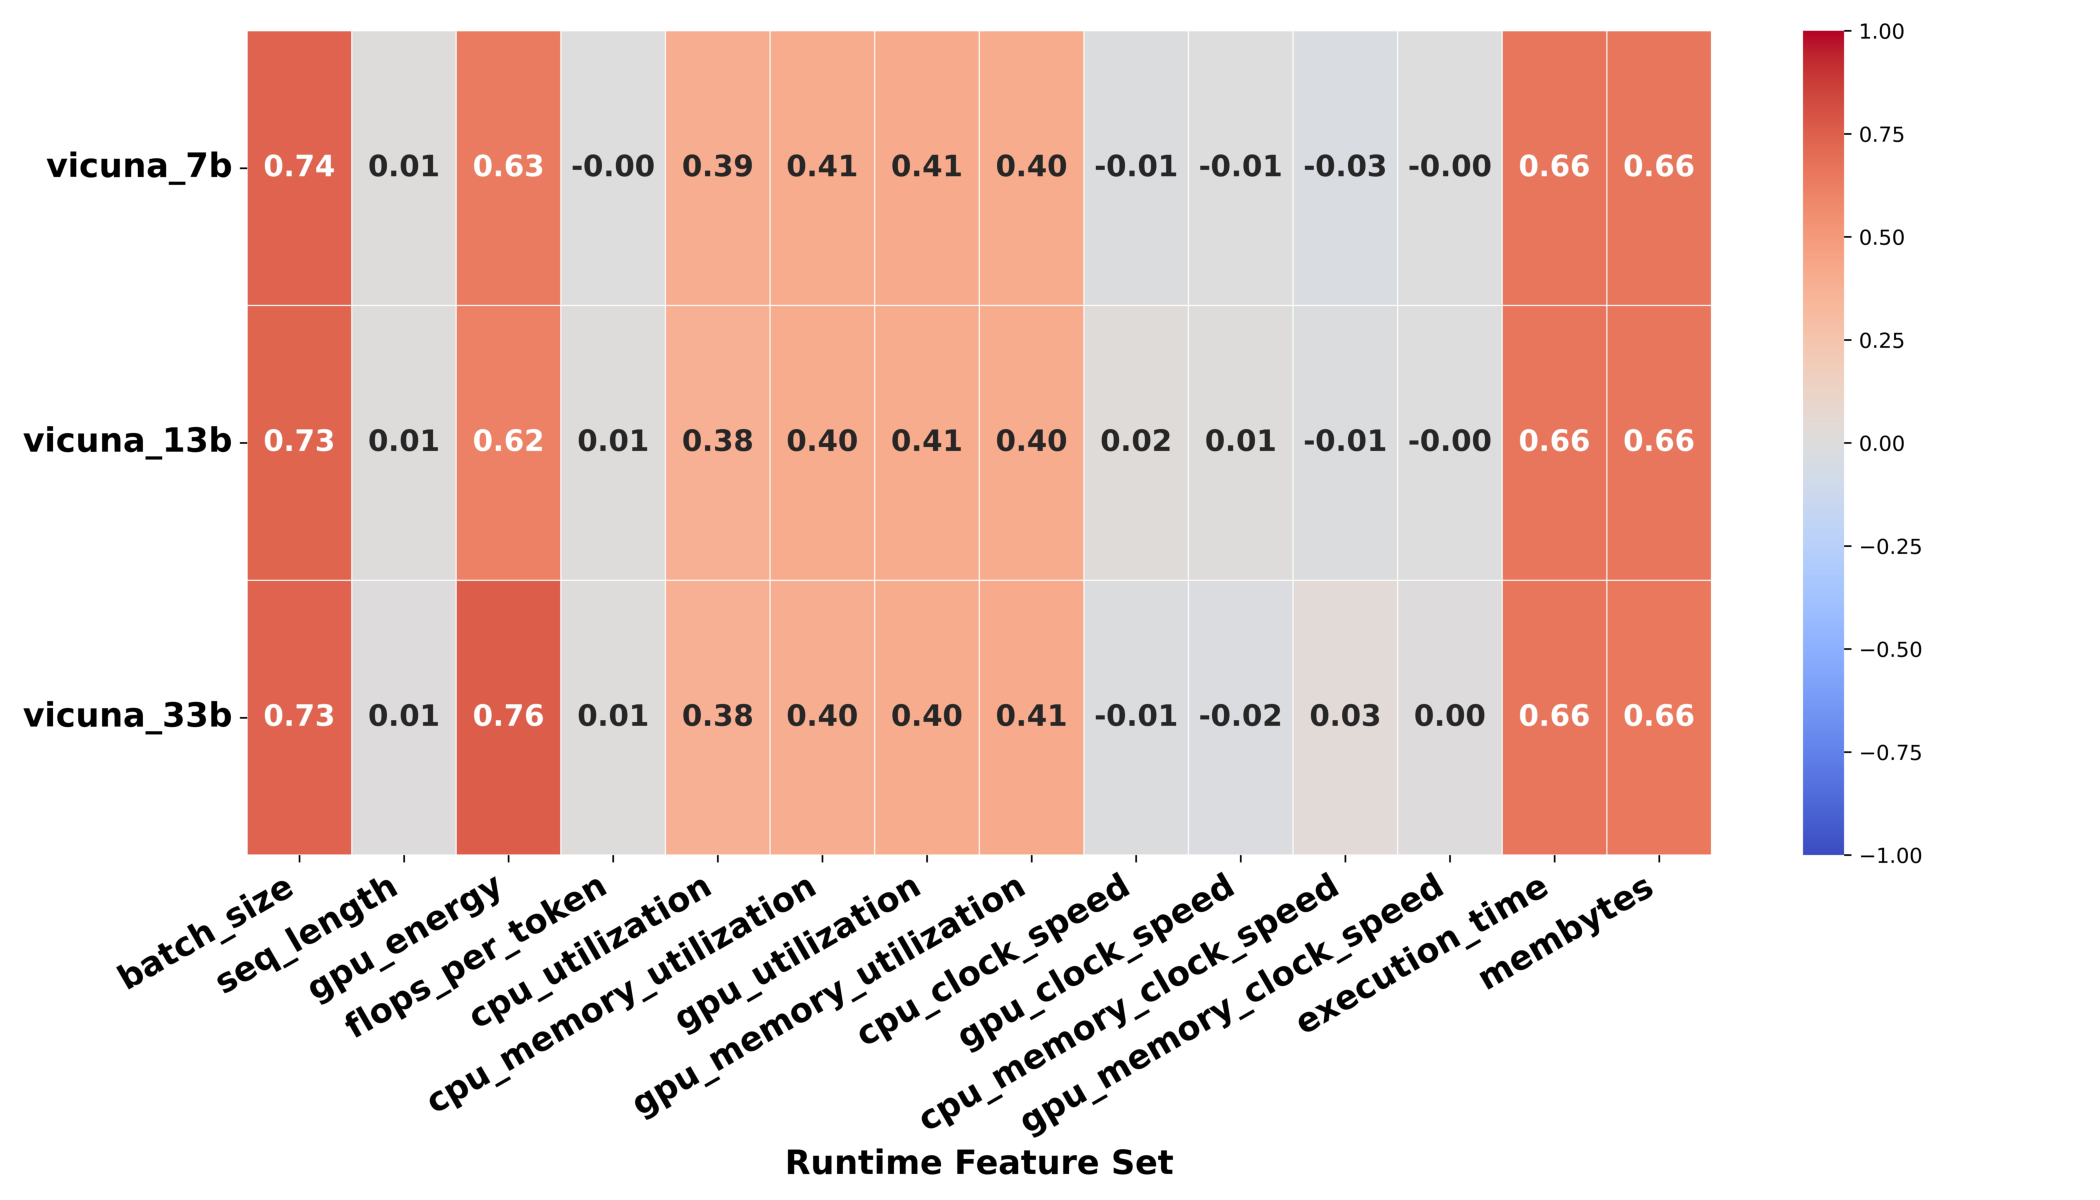
\includegraphics[width=\columnwidth]{figures/vicuna_energy_correlations_4GPU.pdf}
% \caption{Spearman correlation heatmap of runtime features for the Total Model Energy of the 3 Vicuna models with the runtime features.}
% \label{fig:correlation_heatmap}
% % \vspace{-6pt}
% \end{figure}



To assess the influence of different input features on total energy consumption, we performed a Spearman rank correlation analysis across all model configurations for Vicuna. %As shown in Figure~\ref{fig:correlation_heatmap}, GPU energy reported by NVML exhibits a strong correlation with total energy ($\rho$ between $0.633$ and $0.762$), as expected since GPU computation dominates energy consumption in LLMs. 

GPU energy reported by NVML exhibits a strong correlation with total energy ($\rho$ between $0.633$ and $0.762$), as expected since GPU computation dominates energy consumption in LLMs. 
However, other features also show substantial correlations with total energy consumption. Runtime features are particularly strongly correlated with total energy, with batch size ($\rho$ between $0.735$ and $0.737$), execution time ($\rho$ between $0.658$ and $0.664$), and Memory ($\rho$ between $0.656$ and $0.663$) all showing strong correlations. 

These results further demonstrate that apart from GPU energy other system-level utilization metrics also capture critical aspects of energy consumption - particularly in tensor-parallel configurations where communication and synchronization overheads are significant. 



% \section{Ground Truth Energy vs Inference Time plot}
% \label{app:ground-truth-energy}

% \begin{figure}[!t]
% \centering
% % 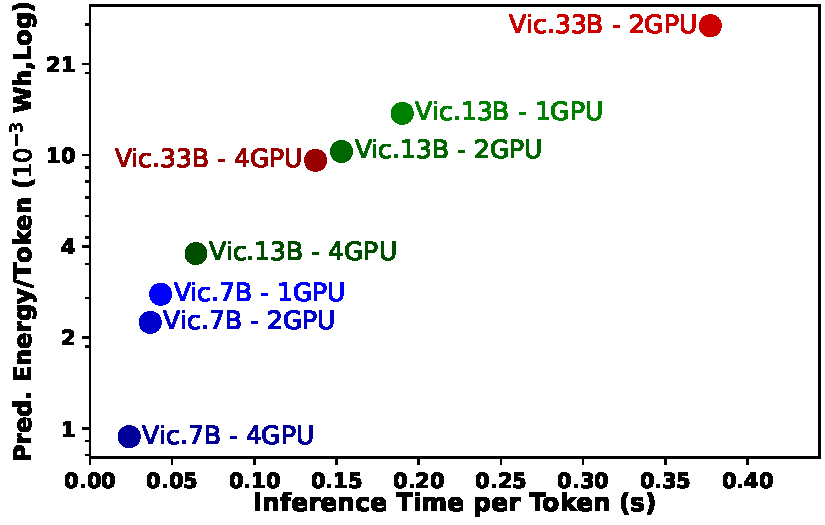
\includegraphics[width=\columnwidth]{figures/pareto_plot.pdf}

% \caption{Actual energy per token vs. inference time per token (log scale) for Vicuna models.\anshul{use wrapfig here too, such a big figure looks bad. make y-axis range same as use case figure else it seems our predictions are significantly off.}}
% \label{fig:pareto_plot_ground_truth}
% % \vspace{-6pt}
% \end{figure}

% Figure~\ref{fig:pareto_plot_ground_truth} shows the trade-off between actual energy consumption and inference time per token across Vicuna model sizes and GPU configurations.
% This is discussed in the context of generalization within the optimal model selection use case in Section~\ref{sec:usecase}.



% \section{Ablation: Role of Model Features}
% \label{app:ablation}

% To assess the contribution of model structure features (e.g. attention heads, feed-forward dimension etc.), we perform an ablation by removing them from the prediction model and comparing MAPE with and without these features for all the variants of Vicuna.
% \begin{table}[t]
% \centering
% \small
% \setlength{\tabcolsep}{4pt}
% \renewcommand{\arraystretch}{1.05}

% \begin{tabular}{
%   @{}
%   l
%   c
%   c
%   @{}
% }
% \toprule
% \textbf{Model} & \textbf{With Model} & \textbf{Without Model} \\
% \textbf{Variant} & \textbf{Features} & \textbf{Features} \\
% \midrule
% \rowcolor{rowblue} Vicuna 7B  & 15.84\% & 17.2\% \\
% Vicuna 13B                    & 17.72\% & 18.2\% \\
% \rowcolor{rowblue} Vicuna 33B & 17.55\% & 20.1\% \\
% \bottomrule
% \end{tabular}

% \caption{Leave-one-out model-level prediction MAPE on NVIDIA A6000 GPUs with and without model features.}
% \label{tab:ablation_model_features}
% \end{table}





% As shown in Table~\ref{tab:ablation_model_features}, while overall prediction accuracy remains similar in full-data settings,
% the inclusion of model features improves generalization performance in leave-one-out evaluations—reducing MAPE by 2–4\% across Vicuna variants. These results suggest that model features help the regressors capture structural differences between variants, improving robustness when extrapolating to unseen configurations. Although the effect on raw prediction accuracy is modest, the improvement in generalization justifies their inclusion in the final model.

\section{Additional Results: Using Latency Prediction Approaches to Predict Energy}
\label{app:latency-ablation}
We evaluate whether a latency-prediction-style approach can be repurposed for energy prediction. 
Specifically, we implement a NeuSight-style baseline for energy prediction~\cite{neusight}. 
NeuSight is a recent latency-prediction framework that decomposes model execution into fine-grained matrix tiles, extracts computational features such as FLOPs and memory behavior, and trains a Multi-Layer Perceptron (MLP) to predict latency. 
We keep the same decomposition and prediction structure, but replace the prediction target with measured system energy. 
This directly tests whether latency-oriented execution features are sufficient for energy prediction.

\begin{table}[t]
\centering
\small
\setlength{\tabcolsep}{6pt}
\renewcommand{\arraystretch}{1.05}

\begin{tabular}{l|c}
\hline
\textbf{Model} & \textbf{MAPE} \tabularnewline
\hline
\rowcolor{rowblue} Vicuna 7B  & 79.19\% \tabularnewline
Vicuna 13B                    & 93.24\% \tabularnewline
\rowcolor{rowblue} Vicuna 33B & 89.38\% \tabularnewline
\hline
\end{tabular}
\vspace{-6pt}
\caption{MAPE for a NeuSight-style latency prediction framework when energy is used as the prediction target.}
\vspace{-6pt}
\label{tab:neusight_energy_target}
\end{table}

Table~\ref{tab:neusight_energy_target} shows that directly substituting energy as the prediction target performs poorly, with an average MAPE of 87.3\%. 
This corresponds to roughly $\sim$3-5$\times$ worse prediction accuracy than \sys{} and $\sim$1-2$\times$ worse accuracy than the least accurate energy-prediction baseline in our evaluation. 
This result shows that energy prediction is not simply latency prediction with a different target label. 
Latency-oriented features capture how long kernels execute, but they do not sufficiently capture the power dynamics, communication overheads, and synchronization effects that determine total system energy during parallel inference.

% \subsubsection{Extending latency prediction techniques to energy}
% %
% \aruna{can be removed, content is moved to main text}
% To demonstrate that latency prediction is not directly analogous to energy prediction, we extend the NeuSight work~\cite{neusight} by a one-to-one substitution of the prediction target  from latency to energy. 
% We choose NeuSight because it is a recent (2025) latency prediction framework that, like \sys{}, decomposes model execution (into fine-grained matrix tiles) and re-composes them to predict end-to-end performance.
% NeuSight captures computational metrics such as FLOPs and memory during execution, and trains a Multi-Layer Perceptron (MLP) to predict latency.
% %\arunacomment{Add something about why you chouse Neusight. May be this is more recent work?}  
% We capture ground truth energy during execution to train the MLP and predict the energy of an unseen test set using the same framework. 

% Our results in Table~\ref{tab:tiling_analogous_4gpu} show that a direct substitution of the prediction target in NeuSight from latency to energy leads to $\sim$3-5$\times$ worse prediction accuracy compared to \sys{} and $\sim$1-2$\times$ worse accuracy compared to the least accurate energy prediction baseline we tested. 



% \begin{table}[t]
% \centering
% \small
% \setlength{\tabcolsep}{6pt}
% \renewcommand{\arraystretch}{1.1}

% \begin{tabular}{l|c}
% \hline
% \textbf{Model} & \textbf{MAPE} \\
% \hline
% \rowcolor{rowblue} Vicuna 7B  & 79.19\% \\
% Vicuna 13B                   & 93.24\% \\
% \rowcolor{rowblue} Vicuna 33B & 89.38\% \\
% \hline
% \end{tabular}

% \caption{MAPE results for NeuSight~\cite{neusight} based prediction with energy as the predictor target.}
% \label{tab:tiling_analogous_4gpu}
% \end{table}


\begin{table}[t]
\centering
\small
\setlength{\tabcolsep}{5pt}
\renewcommand{\arraystretch}{1.05}

\begin{tabular}{lclc}
\toprule
\textbf{Model} & \textbf{MAPE} & \textbf{Model} & \textbf{MAPE} \tabularnewline
\midrule
\rowcolor{rowblue} Vicuna 7B  & 13.34\% & Llama 7B  & 15.30\% \tabularnewline
Vicuna 13B                    & 13.78\% & Llama 13B & 16.51\% \tabularnewline
\rowcolor{rowblue} Vicuna 33B & 14.45\% & Llama 70B & 26.53\% \tabularnewline
Mistral 8B                    & 16.25\% & Qwen 8B   & 16.07\% \tabularnewline
\rowcolor{rowblue} Mistral 24B & 17.25\% & Qwen 14B  & 19.41\% \tabularnewline
Mistral 48B                   & 17.83\% & Qwen 32B  & 14.90\% \tabularnewline
\bottomrule
\end{tabular}

\vspace{-6pt}
\caption{Model-level prediction results for \sys{} on 2$\times$ NVIDIA H200 GPUs.}
\label{tab:h200_model_results}
\vspace{-6pt}
\end{table}


\section{Additional Results on NVIDIA H200 GPUs}
\label{app:additional_perf_results}

Table~\ref{tab:h200_model_results} reports additional model-level prediction results for \sys{} on NVIDIA H200 GPUs. 
These results correspond to the H200 hardware-extension experiment referenced in \S\ref{sec:model_prediction}. 
Across the evaluated model variants, \sys{} achieves an average MAPE of 16.8\%, showing that the same model-tree decomposition and communication- prediction methodology remain effective on a H200s as well.


Table~\ref{tab:h200_module_results} reports module-level prediction results for \sys{} on H200. 
The prediction error remains in the single-digit range across the evaluated modules, including the communication-heavy AllReduce module.

% \vspace{-6pt}

These results provide additional evidence that \sys{} is not tied to a single GPU platform. 
The H200 experiments show that the same decomposition, communication modeling, and structural/runtime feature set can be reused on an additional GPU platform with modest prediction error.

\begin{table}[H]
\centering
\small
\setlength{\tabcolsep}{6pt}
\renewcommand{\arraystretch}{1.05}

\begin{tabular}{lc}
\toprule
\textbf{Module} & \textbf{H200 MAPE} \tabularnewline
\midrule
\rowcolor{rowblue} Self-Attention      & 8.80\% \tabularnewline
MLP                                    & 7.44\% \tabularnewline
\rowcolor{rowblue} AllReduce           & 9.25\% \tabularnewline
LayerNorm/RMSNorm                      & 8.12\% \tabularnewline
\rowcolor{rowblue} LLMEmbedding        & 7.78\% \tabularnewline
\bottomrule
\end{tabular}

\vspace{-6pt}
\caption{Module-level MAPE for \sys{} on NVIDIA H200 GPUs.}
\label{tab:h200_module_results}
\vspace{-6pt}
\end{table}

% \section{Additional Results on NVIDIA B40 and H100 GPUs}
% \label{app:additional_perf_results}

% {To further evaluate whether PIE-P remains effective beyond the primary GPU platform used in our main experiments, we extend our evaluation to two additional GPU platforms: NVIDIA~B40 and NVIDIA~H100. These experiments serve as hardware-extension studies, showing that PIE-P's module-level decomposition and feature-based prediction remain accurate when the underlying GPU architecture and runtime behavior change.}

% {The B40 results show that PIE-P continues to provide accurate fine-grained energy estimates across the major modules of transformer inference. At the module level, PIE-P achieves single-digit MAPE across the main compute and communication components: 7.8\% for Self-Attention, 6.6\% for MLP, 8.2\% for AllReduce, 7.2\% for LayerNorm, and 6.9\% for Embedding. These results show that the predictor is not only fitting end-to-end model energy, but also preserving accuracy at the level of the individual modules used by the model-tree abstraction. In particular, the low AllReduce error on B40 indicates that the communication-aware component of PIE-P remains effective under a different GPU platform.}

% % {We also evaluate leave-one-out generalization on B40 in the 2-GPU setting across multiple model families. For Vicuna, the held-out model errors are 11.83\%, 12.22\%, and 12.81\% for the 7B, 13B, and 33B variants, respectively. Mistral shows slightly higher but still moderate errors of 14.41\%, 15.29\%, and 15.81\% across its variants. Llama shows 13.56\% and 14.64\% for the 7B and 13B models, while the larger 70B model is more challenging at 23.52\%. Qwen achieves 14.25\%, 17.21\%, and 13.21\% across its 8B, 14B, and 32B variants.}

% \aruna{Please add a table for H100 results, no need for leave-one-out I think. }
% {For the 2-GPU H100 setting, PIE-P shows a modest increase in prediction error relative to B40, with each corresponding MAPE value increased by 12.8\%. At the module level, PIE-P obtains 8.80\% for Self-Attention, 7.44\% for MLP, 9.25\% for AllReduce, 8.12\% for LayerNorm, and 7.78\% for Embedding. Despite the increase, the module-level errors remain in the single-digit range, indicating that the same communication-aware decomposition continues to capture the major sources of energy consumption on H100.}

% {The leave-one-out results on H100 also remain moderate in the 2-GPU setting. For Vicuna, the held-out model errors are 13.34\%, 13.78\%, and 14.45\% for the 7B, 13B, and 33B variants, respectively. Mistral obtains 16.25\%, 17.25\%, and 17.83\% across its variants. Llama obtains 15.30\% and 16.51\% for the 7B and 13B models, while the larger 70B model reaches 26.53\%. Qwen obtains 16.07\%, 19.41\%, and 14.90\% across its 8B, 14B, and 32B variants. These results suggest that while H100 introduces somewhat higher prediction error, PIE-P's feature-based and communication-aware design remains effective across GPU platforms.}

% {For the 4-GPU B40 setting, PIE-P again maintains reasonable accuracy across families. Vicuna obtains 14.21\%, 13.39\%, and 15.25\% MAPE across the 7B, 13B, and 33B variants. Mistral obtains 16.66\%, 19.29\%, and 19.71\%, while Qwen obtains 14.54\%, 16.34\%, and 14.91\%. Taken together, these results provide additional evidence that PIE-P is not tied to a single GPU platform. Although a fully hardware-agnostic predictor remains future work, the B40 and H100 experiments show that the same decomposition, communication modeling, and structural/runtime feature set can be reused successfully on additional GPU platforms with modest prediction error.}






% Requires the same packages/macros as the existing appendix tables:
% \usepackage{booktabs}
% \usepackage[table]{xcolor}
% \usepackage{array}
% and an existing rowblue definition.


% \begin{table}[t]
% \centering
% \small
% \setlength{\tabcolsep}{3pt}
% \renewcommand{\arraystretch}{1.05}

% \begin{tabular}{
% @{}
% l
% c
% l
% c
% @{}
% }
% \toprule
% \textbf{Model} & \textbf{MAPE} & \textbf{Model} & \textbf{MAPE} \\
% \midrule
% \rowcolor{rowblue} Vicuna 7B   & 41.1\% & Llama 7B   & 53.1\%  \\
% Vicuna 13B                     & 48.3\% & Llama 13B  & 51.2\%  \\
% \rowcolor{rowblue} Vicuna 33B  & 52.8\% & Llama 70B  & 112.5\% \\
% \midrule
% Mistral 8B                     & 41.2\% & Qwen 8B    & 38.4\%  \\
% \rowcolor{rowblue} Mistral 24B & 43.4\% & Qwen 14B   & 39.9\%  \\
% Mistral 48B                    & 43.8\% & Qwen 32B   & 41.1\%  \\
% \bottomrule
% \end{tabular}

% \caption{MAPE when using NVML-reported GPU energy as a proxy for total system energy on NVIDIA B40 GPUs. This approach produces substantially higher errors compared to \sys{}.}
% \label{tab:b40_nvml_proxy}
% \end{table}


% \begin{table}[t]
% \centering
% \small
% \setlength{\tabcolsep}{3pt}
% \renewcommand{\arraystretch}{1.05}

% \begin{tabular}{
% @{}
% l
% c
% l
% c
% @{}
% }
% \toprule
% \textbf{Model} & \textbf{MAPE} & \textbf{Model} & \textbf{MAPE} \\
% \midrule
% \rowcolor{rowblue} Vicuna 7B   & 63.6\% & Llama 7B   & 71.4\%  \\
% Vicuna 13B                     & 62.3\% & Llama 13B  & 79.3\%  \\
% \rowcolor{rowblue} Vicuna 33B  & 68.9\% & Llama 70B  & 115.2\% \\
% \midrule
% Mistral 8B                     & 48.3\% & Qwen 8B    & 63.1\%  \\
% \rowcolor{rowblue} Mistral 24B & 61.2\% & Qwen 14B   & 68.2\%  \\
% Mistral 48B                    & 61.9\% & Qwen 32B   & 65.5\%  \\
% \bottomrule
% \end{tabular}

% \caption{Leave-one-out generalization results for NVML-based regression on NVIDIA B40 GPUs. Each row shows MAPE when using NVML measurements to predict total energy for a model excluded from training.}
% \label{tab:b40_nvml_loo}
% \end{table}



% \anurag{ablation for methodology - maybe predict directly the  model energy}
% \anurag{ablation for communication modelling methodology}
% \anurag{tables for h100 results}
% \anurag{additional writeup for the B40 results in the main result/evaluation section}
